\documentclass[
	%a4paper, % Use A4 paper size
	letterpaper, % Use US letter paper size
]{jdf}

\addbibresource{references.bib}

\author{Mohamed Fayed, Kruthik Ravikanti, Bruce Walker}
\email{mohamed.fayed@gatech.edu, kravikanti3@gatech.edu, bruce.walker@psych.gatech.edu}
\title{Chart-to-Table Conversion: A Survey}

\begin{document}
%\lsstyle

\maketitle

\begin{abstract}
    Multimodal     Large Language Models (MLLMs) have shown impressive visual capabilities in many Visual Question Answering tasks.
In this paper, we aim to survey the recent advancements in Chart-to-Table task, score the performance of some MLLMs and highlight their strengths and weaknesses.
Our quantitative and qualitative analysis shows that there is a room for improvmenet in Chart-to-Table conversion.
     \end{abstract}

     \tableofcontents

\section{Introduction}\label{sect:intro}
Chart-to-Table is the task of extracting data points from an image of a chart into a table usually in markdown\cite{liu2022deplot;masry2024chartgemma}.
This task is important in the process of digitizing those charts into more space efficient format of text.
Moreover, tables are more accessible mean of communicating data to people with disabilities who count on screen readers in interacting with digital world.

%\section{Related Work}
There has been a lot of efforts in summarizing charts, answering questions~\cite{masry2022chartqa,masry2024chartgemma} and converting them into tables~\cite{liu2022deplot}.
Recently, there has been efforts to analyze the performance of Multimodal Large Language Models (MLLMs) in many all of those tasks.
In our work, we aim to pay closer attention to Chart-to-Table task.
Our main contributions are:
\begin{enumerate}
         \item Survey recent advancements in Chart-to-Table task,
         \item Do quantitative analysis for some models on different benchmark datasets,
         \item Do fine-grained qualitative analysis on various kinds of charts, and
         \item highlight strengths, weaknesses and rooms for improvement of those models in performing this task
              \end{enumerate}
\section{Methodology}\label{sect:methodology}
\subsection{Datasets}
In our analysis, we focus on reporting scores on testsets of ICPR22~\cite{rousseau2023pattern} and PlotQA~\cite{methani2020plotqa} datasets.
ICPR22 testset~\cite{rousseau2023pattern} is gathered from research papers published on PubMed Central website.\footnote{\href{https://pmc.ncbi.nlm.nih.gov}{https://pmc.ncbi.nlm.nih.gov}}
Those publications are in biomedical and life sciences domains.
It contains 443 charts splitted into 5 types: Line Charts, Horizontal and Vertical Bar Charts, Scatter Plot and Vertical Box Plot.

PlotQA~\cite{methani2020plotqa} was made by gathering data from various online sources, such as World Bank and Open Data, generate plots out of these data points, and ask annotators questions about those provided charts.
In our work, we focus on the data points used in constructing the charts only.
Its test set contains 33657 charts divided equally among dotted line charts, line charts, and vertical and horizontal bar charts.
In our analysis, due to limitations on API calls and time constraints, we ran computed scores for 3000 randomly selected charts.

\subsection{Models}\label{ssect:models}
For our analysis, we selected the following models:
\begin{itemize}
    \item Gemini 1.5 Flash~\cite{team2024gemini}: A general purpose lightweight MLLM.
         \item ChartGemma~\cite{masry2024chartgemma}: A specialized model in chart summarization, question answering and reasoning about charts.
             It utilizes PaliGemma~\cite{beyer2024paligemma} as its backbone, and was tuned on Visual Chart Instructions dataset.
         \item Deplot~\cite{liu2022deplot}: An encoder-decoder model based on Matcha~\cite{liu2022matcha} that is specialized in converting charts into tables.
              \end{itemize}
\subsection{Evaluation}
\begin{itemize}
    \item Relative Mapping Similarity (RMS)
    \item Qualitative
              \end{itemize}

\section{Results and Discussion}\label{sect:qualitative-analysis}
\subsection{Relative Mapping Similarity Scores}\label{ssect:rms}
\subsection{Text Recognition}\label{ssect:qualitative-text-recognition}
For the sample we analyzed, there has been no errors in recognizing text in the images, e.g. columns names.
However, table~\ref{tab:charggemma-plotqa-line-21673} shows that ChartGemma has a tendency to labelize even if there are no labels in the input image.
\footnote{the prediction of Gemini and Ground Truth have no labels for x-axis, but ChartGemma made years as labels.}
\footnote{In some cases, the ground truth is mislabelled. The reference has no values for x-axis, but the image includes them as in~\ref{fig:plotqa-line-20049}.}
For both models, the tables layouts were perfectly generated into table in json format for Gemini and markdown for ChartGemma.

\subsection{Values Extraction}\label{ssect:values-extraction}
For PlotQA and ICPR22 samples, it is frequent to find errors like:
\begin{enumerate}
         \item rounding errors, e.g. $15.42->15 and 15.6->15$.
         \item Precision Errors: we have noticed that the model can not predict more than 3 digits for each value, e.g. $126765000.0->156000000$.
         \item In case of near values, e.g. $24.18, 24.09$, there might be some errors, e.g. predicting $23$ instead of $24$.
             For that kind of error, it may result in changing trend, e.g. steady performance may seam as decreasing.
             \footnote{It is worth noting that we have not seen cases where increasing is replaced by decreasing trends or vice versa.}
             \item Gemini can differentiate outputs based on scale, e.g. $156000000 \& 50.2$ for instance.
                 However, both models sometimes change scale, e.g. table~\ref{tab:chartgemma-plotqa-line-21673} where ChartGemma returned values multiplied by 10.
             \item Occasionally, both models swap two columns as shown in table~\ref{tab:gemini-plotqa-line-18806}.
                 As a result, RMS score is significantly lower (f1=0.34) than its fixed version (f1=0.83).
              \end{enumerate}

              In the following subsubsections, we illustrate issues related to each kind of graphs.

\subsubsection{Bar Charts}\label{sssect:bar-errors}
\begin{enumerate}
    \item Tables~\ref{tab:chartgemma-plotqa-vbar-21673} and~\ref{tab:gemini-plotqa-vbar-21673} show that both models are very good in extracting data points from bar charts.
        \footnote{A small notice, that needs more examples to approve/disapprove, is that ChartGemma has lower margin of error while having less precision. The numbers of Canada, for instance, are correctly approximated to 52. This may indicate almost steady value, which sounds reasonable conclusion for that country, especially when looking to the whole graph at a glance.}
              \end{enumerate}
              \subsubsection{Line Charts}\label{sssect:line-errors}
              \begin{enumerate}
         \item There are some graphs, like~\ref{fig:icpr22-line-6339}, the Gemini API just fails with no clear response message (till now).
             However, it is suspected that the very large number of data points might be the reason.
         \item Table~\ref{tab:chartgemma-plotqa-line-20049} shows that ChartGemma may fail in extracting data points from slightly complex graphs.
             It fails in both extracting correct values as well as mapping them to the correct label.
                            \end{enumerate}
              Tables~\ref{tab:gemini-plotqa-vbar-25905} and~\ref{tab:chartgemma-plotqa-vbar-25905} include Gemini 1.5 Flash and ChartGemma predictions for figure~\ref{fig:plotqa-vbar-25905} respectively.
\begin{figure}
     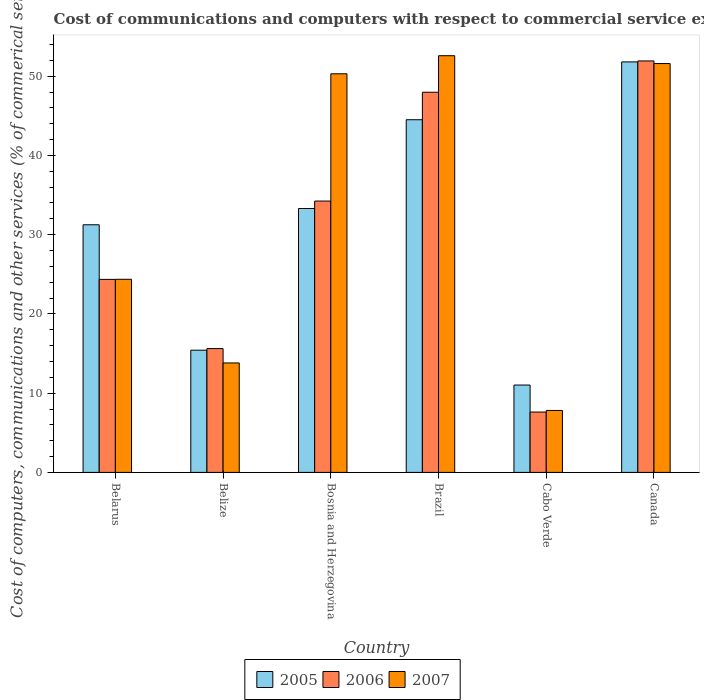
\includegraphics{test-sample/plotqa/images/vertical-bar/25905.png}
     \caption{Vertical Bar Chart example from PlotQA testset.}\label{fig:plotqa-vbar-25905}
      \end{figure}
\begin{table}
    \begin{tabular}{llrrr}
\toprule
 & Country & 2005 & 2006 & 2007 \\
\midrule
0 & Belarus & 31 & 24 & 23 \\
1 & Belize & 15 & 15 & 13 \\
2 & Bosnia and Herzegovina & 33 & 34 & 52 \\
3 & Brazil & 44 & 47 & 52 \\
4 & Cabo Verde & 10 & 7 & 8 \\
5 & Canada & 51 & 52 & 51 \\
\bottomrule
\end{tabular}
    \caption{Gemini 1.5 Flash predictions on Vertical Bar \# 25905}
    \label{tab:gemini-plotqa-vbar-25905}
\end{table}

\begin{table}
\begin{tabular}{lllll}
\toprule
 & Country  & 2005 Cost of computers, communications and other services ($\%$ of commerical service exports)  & 2006 Cost of computers, communications and other services ($\%$ of commerical service exports)  & 2007 Cost of computers, communications and other services ($\%$ of commerical service exports)  \\
\midrule \\
1 & Belarus  & 31  & 24  & 24  \\
2 & Belize  & 15  & 15  & 13  \\
3 & Bosnia and Herzegovina  & 33  & 35  & 49  \\
4 & Brazil  & 45  & 47  & 53  \\
5 & Cabo Verde  & 11  & 8  & 8  \\
6 & Canada  & 52  & 52  & 52  \\
\bottomrule
\end{tabular}
    \caption{ChartGemma predictions for vertical bar image no. 2590 from PlotQA}
    \label{tab:chartgemma-plotqa-vbar-25905}
\end{table}


\begin{figure}
     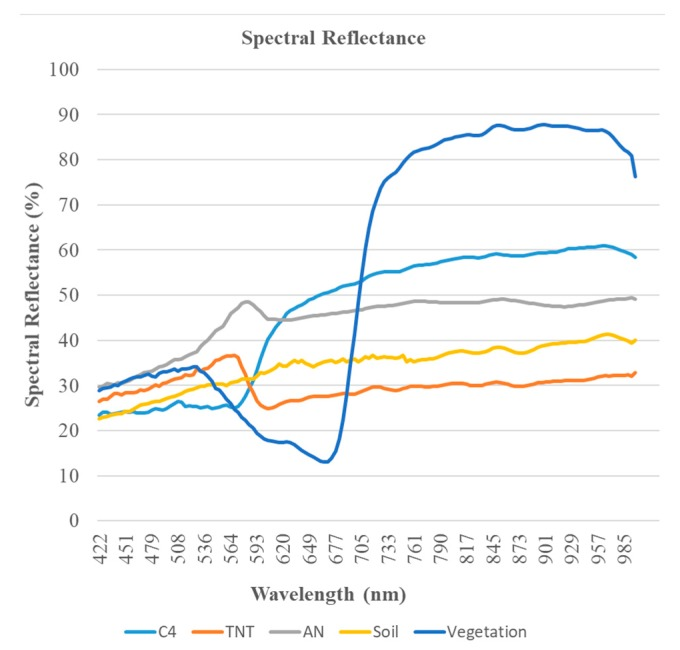
\includegraphics{test-sample/icpr22/images/line/PMC6339093___05.jpg}
     \caption{Example for charts that causes the API to fail.}
     \label{fig:icpr22-line-6339}
      \end{figure}
\begin{figure}
     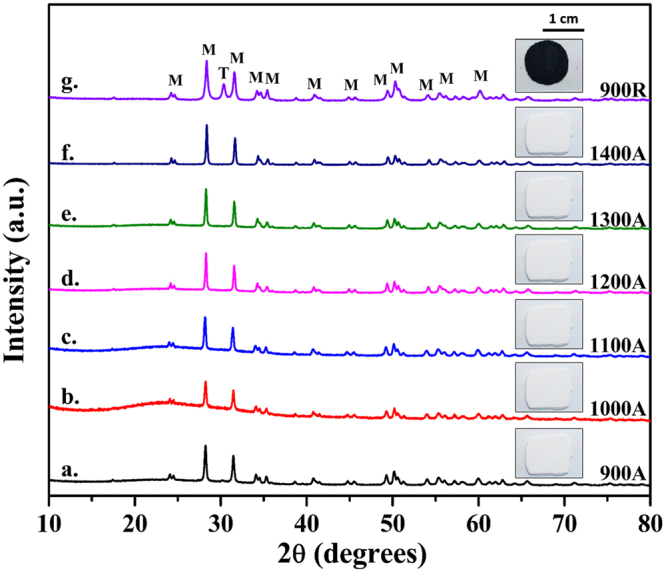
\includegraphics{test-sample/icpr22/images/line/PMC5882956___1_HTML.jpg}
     \caption{A good example for graph in the wild that causes Gemini 1.5 Flash to fail.}
     \label{fig:icpr22-line-5882}
      \end{figure}
\begin{figure}
     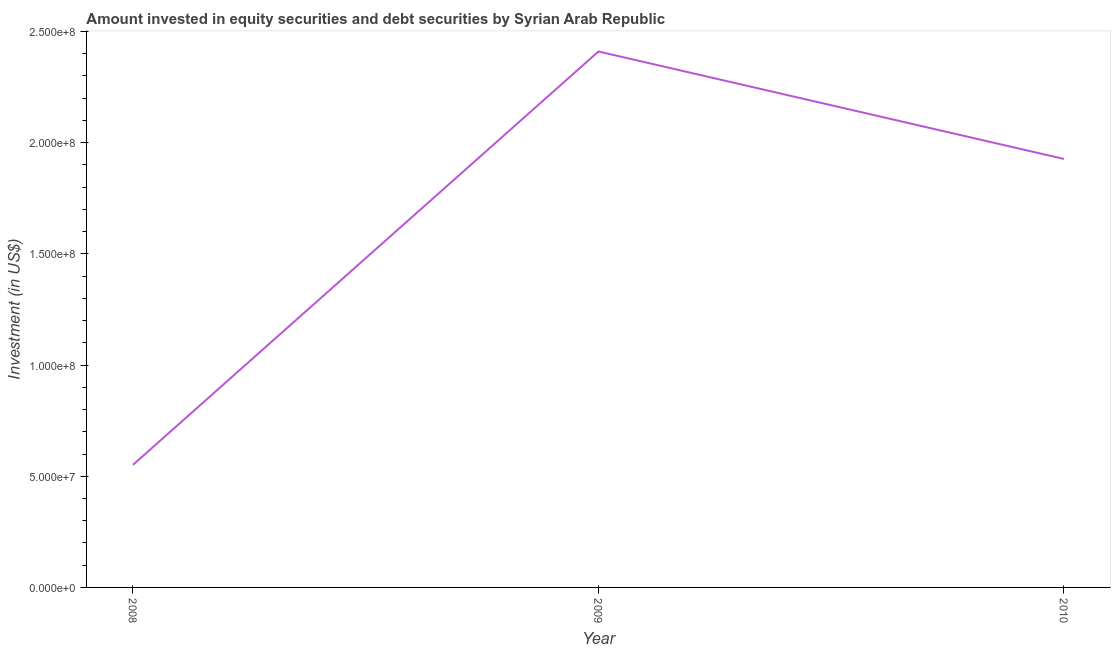
\includegraphics{test-sample/plotqa/images/line/21673.png}
     \caption{Example for Line Chart from PlotQA testset \# 21673 about Portfolio Investment}
     \label{fig:plotqa-line-21673}
      \end{figure}
\begin{table}
\begin{tabular}{lllllll}
\toprule
 & name & color & label & bboxes & y & x \\
\midrule
0 & Portfolio Investment & \#BA55D3 & Portfolio Investment & [{'y': 51, 'x': 132, 'w': 466, 'h': 413}, {'y': 51, 'x': 598, 'w': 465, 'h': 107}] & [55132083.68, 241005430.1, 192682327.3] & [0, 1, 2] \\
\bottomrule
\end{tabular}
     \caption{Reference for Line Chart from PlotQA \#21673 Portfolio Investment}
     \label{tab:plotqa-line-21673-ref}
\end{table}

\begin{table}
    \begin{tabular}{lrr}
\toprule
 & Year & Investment (in USD) \\
\midrule
0 & 2008 & 54000000 \\
1 & 2009 & 240000000 \\
2 & 2010 & 200000000 \\
\bottomrule
\end{tabular}
     \caption{Predicted data points by Gemini 1.5 Flash for Line Chart from PlotQA \#21673 Portfolio Investment}
     \label{tab:plotqa-line-21673-gemini-flash}
     \end{table}

\begin{table}
\begin{tabular}{lll}
\toprule
 & Year  & Investment (in USD)  \\
\midrule
1 & 2008  & 500000000  \\
2 & 2009  & 2400000000  \\
3 & 2010  & 1900000000  \\
\bottomrule
\end{tabular}
    \caption{ChartGemma: prediction for PlotQA line chart \#21673}
    \label{tab:chartgemma-plotqa-line-21673}
\end{table}


\begin{figure}
     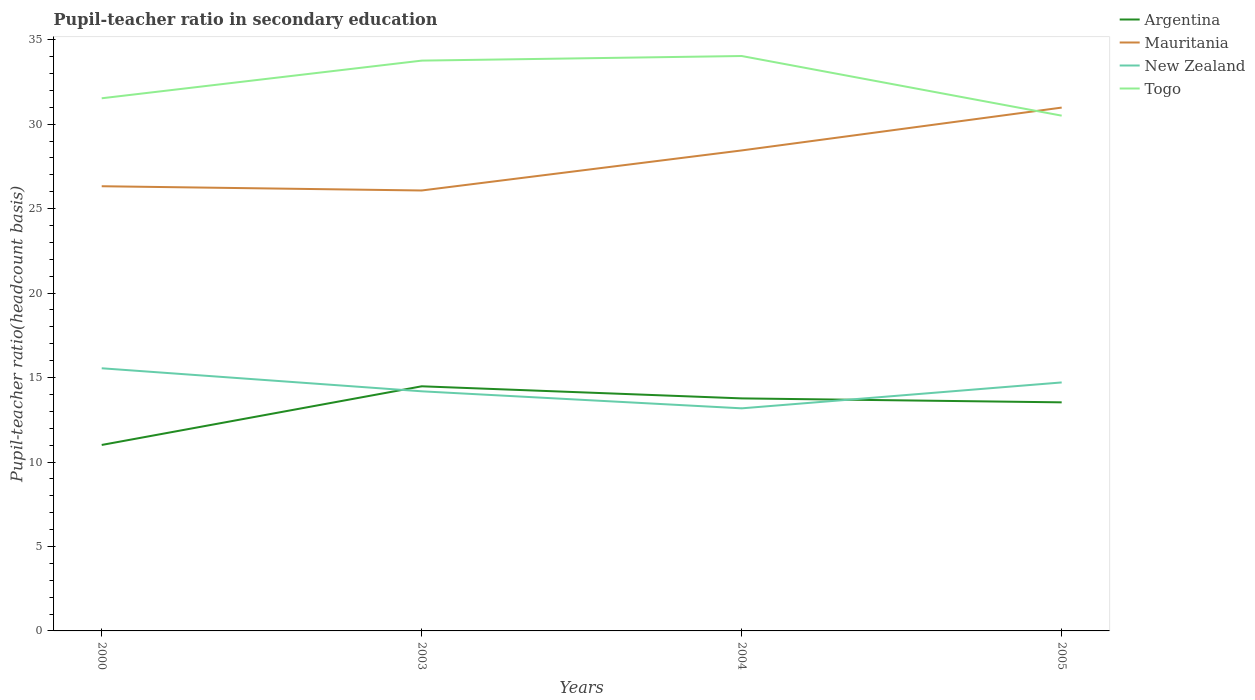
\includegraphics{test-sample/plotqa/images/line/20049-4-lines.png}
     \caption{PlotQA \# 20049: Line chart containing 4 lines.}\label{fig:plotqa-line-20049}
      \end{figure}
      \begin{table}
\begin{tabular}{lllllll}
\toprule
 & name & color & label & bboxes & y & x \\
\midrule
0 & Argentina & \#228B22 & Argentina & [{'y': 386, 'x': 101, 'w': 320, 'h': 58}, {'y': 386, 'x': 421, 'w': 320, 'h': 12}, {'y': 398, 'x': 741, 'w': 320, 'h': 4}] & [11.0102100372314, 14.4826498031616, 13.7663202285767, 13.5325899124146] & [0, 1, 2, 3] \\
1 & Mauritania & \#CD853F & Mauritania & [{'y': 186, 'x': 101, 'w': 320, 'h': 4}, {'y': 150, 'x': 421, 'w': 320, 'h': 40}, {'y': 107, 'x': 741, 'w': 320, 'h': 43}] & [26.3266506195068, 26.0756893157958, 28.4472198486328, 30.9836406707764] & [0, 1, 2, 3] \\
2 & New Zealand & \#66CDAA & New Zealand & [{'y': 368, 'x': 101, 'w': 320, 'h': 23}, {'y': 391, 'x': 421, 'w': 320, 'h': 17}, {'y': 382, 'x': 741, 'w': 320, 'h': 26}] & [15.5497102737427, 14.1861000061035, 13.1779899597168, 14.7109498977661] & [0, 1, 2, 3] \\
3 & Togo & \#90EE90 & Togo & [{'y': 60, 'x': 101, 'w': 320, 'h': 38}, {'y': 56, 'x': 421, 'w': 320, 'h': 4}, {'y': 56, 'x': 741, 'w': 320, 'h': 59}] & [31.5344390869141, 33.7643890380859, 34.03617858886719, 30.5053195953369] & [0, 1, 2, 3] \\
\bottomrule
\end{tabular}
    \caption{Reference table for PlotQA line chart \# 20049}
    \label{tab:ref-plotqa-line-20049}
\end{table}

      \begin{table}
    \begin{tabular}{lrrrrr}
\toprule
 & Year & Argentina & Mauritania & New Zealand & Togo \\
\midrule
0 & 2000 & 10.600000 & 26.000000 & 15.800000 & 31.400000 \\
1 & 2003 & 14.200000 & 25.800000 & 14.000000 & 33.200000 \\
2 & 2004 & 13.600000 & 28.000000 & 13.000000 & 33.800000 \\
3 & 2005 & 13.400000 & 30.200000 & 14.600000 & 30.000000 \\
\bottomrule
\end{tabular}
    \caption{Gemini 1.5 Flash prediction for PlotQA line chart \# 20049}
    \label{tab:gemini-plotqa-line-20049}
\end{table}

      \begin{table}
    \begin{tabular}{llllll}
\toprule
 & Years  & Argentina  & Mauritius  & New Zealand  & Togo  \\
\midrule
1 & 2000  & 21  & 15  & 22  & 11  \\
2 & 2003  & 21  & 14  & 23  & 14  \\
3 & 2004  & 22  & 13  & 23  & 13  \\
4 & 2005  & 21  & 14  & 21  & 14  \\
\bottomrule
\end{tabular}
    \caption{ChartGemma prediction for PlotQA line chart \# 20049. The model fails in mapping lines with values, e.g. Togo column seams more likely to be Argentina. For values, it is obvious that ChartGemma is very far away from correctly detecting values greater than 20!}
    \label{tab:chartgemma-plotqa-line-20049}
\end{table}


\begin{table}
\begin{tabular}{llll}
\toprule
 & Australia & Turkmenistan & United States \\
\midrule
0 & {'Year': 2009.0, 'Subscribers per 100 People': 47.0} & {'Year': 2009.0, 'Subscribers per 100 People': 48.5} & {'Year': 2009.0, 'Subscribers per 100 People': 9.0} \\
1 & {'Year': 2010.0, 'Subscribers per 100 People': 46.0} & {'Year': 2010.0, 'Subscribers per 100 People': 47.5} & {'Year': 2010.0, 'Subscribers per 100 People': 10.0} \\
2 & {'Year': 2011.0, 'Subscribers per 100 People': 45.0} & {'Year': 2011.0, 'Subscribers per 100 People': 46.0} & {'Year': 2011.0, 'Subscribers per 100 People': 11.0} \\
3 & {'Year': 2012.0, 'Subscribers per 100 People': 44.5} & {'Year': 2012.0, 'Subscribers per 100 People': 45.0} & {'Year': 2012.0, 'Subscribers per 100 People': 11.5} \\
4 & {'Year': 2013.0, 'Subscribers per 100 People': 44.0} & {'Year': 2013.0, 'Subscribers per 100 People': 44.0} & {'Year': 2013.0, 'Subscribers per 100 People': 12.0} \\
\bottomrule
\end{tabular}
\caption{Example for Gemini Flash predictions where it swapped the values of Turkmenistan and United States. The swapped table has score of $F1=0.34$ and the corrected version has $F1=0.83$.}
\label{tab:gemini-plotqa-line-18806}
\end{table}


\section{Conclusion and Recommendations}\label{sect:conclusion}
In this report, we document our quanitative analysis for LLMs behavior in Chart-to-Table task.
Based on the selected sample, we observed that the model can accurately recognize the layout of the graph, but it is not very precise in recognizing small differences in values.
For future work, we recommend combining both LLMs and Computer Vision algorithms to complement each other in accurately converting charts into tables.
\footnote{Based on my expertise in using LLaMA 3.1 8B Instruct, we can convert among formats with almost no errors, e.g. convert prints from python code in latex table. It correctly follows instruction of to round numerical values or copy them as is.}
\section{References}
\printbibliography[heading=none]
\end{document}
